\documentclass[a4paper, 11pt, final, garamond]{book}
\usepackage{cours-preambule}

\makeatletter
\renewcommand{\@chapapp}{Thermodynamique -- chapitre}
\makeatother

\hfuzz=5.002pt

% \toggletrue{student}
% \toggletrue{corrige}
% \renewcommand{\mycol}{black}
\renewcommand{\mycol}{gray}

\begin{document}
\setcounter{chapter}{0}

\settype{enon}
\settype{solu_prof}
\settype{solu_stud}

\chapter{\cswitch{Correction du TD}{TD~: Systèmes thermodynamiques}}

\resetQ
\section{Pression des pneus}
\enonce{%
	La pression préconisée sur les roues avant d'une Mégane est de \SI{2.2}{bars}.
	On règle la pression des pneus un jour froid de cet hiver, par une température
	extérieure de $\SI{-5}{\degreeCelsius}$.
}%
\QR{%
	En supposant que le volume des pneus ne varie par et qu'il n'y a aucune fuite
	d'air possible, quelle sera l'indication du manomètre un jour chaud cet été,
	par une température extérieure de $\SI{30}{\degreeCelsius}$~?
}{%
	Comme la quantité de matière $n$ d'air contenue dans le pneu et son volume
	sont des constantes, alors d'après l'équation d'état du gaz parfait on a
	\begin{gather*}
		\frac{P_1}{T_1} = \frac{P_2}{T_2} = \frac{nR}{V}
		\\\Lra
		\boxed{P_2 = \frac{T_2}{T_1}P_1}
		\Ra
		\xul{P_2 = \SI{2.5}{bars}}
	\end{gather*}
}%
\QR{%
	Calculer la variation relative de pression due au changement de température.
	Que conseillez-vous~?
}{%
	La variation relative de pression est supérieure à 10\%, ce qui est loin
	d'être négligeable. Le meilleur conseil à donner est de refaire la pression
	des pneus~! Notez par ailleurs qu'il est préconisé de la vérifier chaque mois,
	et \textbf{indispensable} de le faire au moins deux fois par an \textbf{et}
	avant les grands trajets.
}%

\resetQ
\section{Fuite d'hélium}
\enonce{%
	On considère une bouteille de volume constant $V = \SI{10}{L}$ contenant de
	l'hélium, modélisé comme un gaz parfait monoatomique, à la pression $P =
		\SI{2.1}{bars}$ et à la température $T = \SI{30}{K}$.
	\begin{tcn}(data)<lfnt>{Données}
		$M(\ce{He}) = \SI{4.0}{g.mol^{-1}}$, $k_B = \SI{1.38e-23}{J.K^{-1}}$.
	\end{tcn}
}%
\QR{%
	Calculer la masse $m$ d'hélium dans la bouteille, puis la densité particulaire
	$n^*$, c'est-à-dire le nombre d'atomes par unité de volume.
}{%
	solu
}%
\QR{%
	Calculer la vitesse quadratique moyenne des atomes.
}{%
	solu
}%
\QR{%
	À la suite de l'ouverture de la bouteille, la pression passe à $P' =
		\SI{1.4}{bars}$ et la température à $T' = \SI{290}{K}$. Calculer la masse
	$\Delta{m}$ de gaz qui s'est échappé de la bouteille.
}{%
	solu
}%
\QR{%
	On a vite refermé la bouteille. À quelle température $T''$ faudrait-il porter
	le gaz pour atteindre à nouveau la pression $P$~?
}{%
	solu
}%

\resetQ
\section{Gaz parfait dans une enceinte}
\enonce{%
	Une quantité de matière $n$ de gaz parfait est enfermée dans une enceinte de
	surface de section $S$. Cette enceinte est fermée par un piston de masse $m$,
	à même de coulisser sans frottement, et permet les transferts thermiques, si
	bien que lorsqu’on attend suffisamment longtemps le gaz contenu dans
	l’enceinte est en équilibre thermique avec l’extérieur. Le milieu extérieur se
	trouve à température et pression constantes $T_0$ et $P_0$ . On fait subir au
	gaz la série de transformations suivante~:
	\begin{enumerate}[label=\clenumi]
		\item Initialement, dans l'état (1), le système est au repos depuis
		      suffisamment longtemps pour avoir atteint l'équilibre thermique et
		      mécanique~;
		\item État (2)~: le gaz est chauffé jusqu'à ce qu'il atteigne la température
		      $T > T_0$~;
		\item État (3)~: on place brusquement une masse supplémentaire $M$ sur le
		      piston, l'équilibre thermique n'est pas atteint~;
		\item État (4)~: l'équilibre thermique est atteint.
	\end{enumerate}
	\begin{center}
		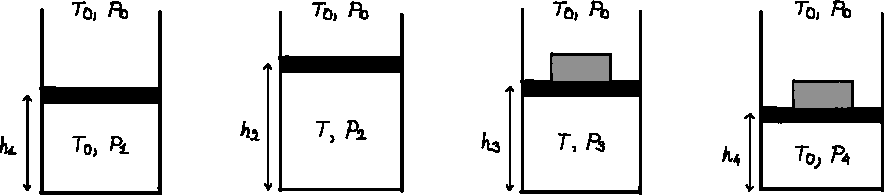
\includegraphics[width=.8\linewidth]{piston-plain}
	\end{center}
}%
\QR{%
	Exprimer les hauteurs $h_1$ à $h_4$ du piston dans chaque état.
}{%
	solu
}%

\resetQ
\section{Ressort à gaz}
\enonce{%
	Les sièges de bureaux sont souvent montées sur un vérin cylindrique permettant
	d'en ajuster la hauteur. On décrit ce vérin cylindrique à air comprimé, supposé
	parfait, par le schéma ci-dessous.
	\begin{center}
		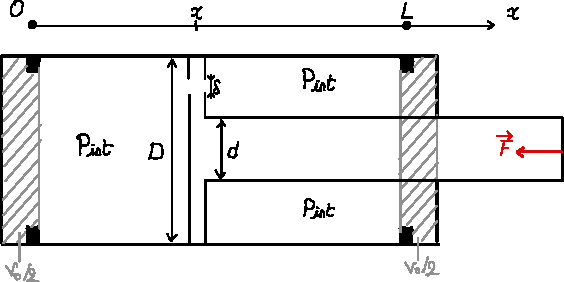
\includegraphics[width=.7\linewidth]{ressort_gaz-plain}
	\end{center}
	Le piston a une épaisseur nulle, et on pourra négliger la section de l'orifice
	de communication de diamètre $\delta $ devant les autres sections. On note $V_0$
	l'ensemble des deux volumes morts que le piston ne peut atteindre, situés en
	$x<0$ et $x>L$. On prendra également $D = 2d$. On supposera que l'équilibre
	thermique du gaz avec l'air extérieur de température $T_0$ est réalisé pour
	toute position du piston, et on note $P_0$ la pression extérieure.
}%
\QR{%
	Exprimer le volume $V(x)$ disponible pour le gaz dans le vérin en fonction de
	$L$, $x$ et $d$.
}{%
	solu
}%
\QR{%
	Donnez l'expression de $p\ind{int}(x)$ en fonction de $V(x)$.
}{%
	solu
}%
\QR{%
	On suppose le système à l'équilibre mécanique avec le piston à la position
	$x$. Une personne s'assoie sur le siège, exerçant une force $\Ff$. Exprimer la
	force $\Ff'$ qu'exerce la tige sur le système extérieur.
}{%
	solu
}%

\resetQ
\section{Recherche d'un état final}
\enonce{%
	\noindent
	\begin{minipage}[c]{.65\linewidth}
		Une enceinte indéformable aux parois calorifugées\ftn{Qui ne laisse pas passer la
			chaleur.} est séparée en deux compartiments par une cloison étanche de surface
		$S$, mobile, diathermane\ftn{Qui laisse passer la chaleur.} et reliée à un
		ressort de constante de raideur $k$. Les deux compartiments contiennent chacun
		un gaz parfait. Dans l’état initial, le gaz du compartiment 1 est dans l’état
		($T_0$, $V_0$, $P_0$, $n$), le gaz du compartiment 2 dans l’état ($T_0$, $V_0$,
		$2P_0$, $2n$), une cale bloque la cloison mobile et la longueur du ressort est
		égale à sa longueur à vide. On enlève la cale et on laisse le système atteindre
		un état d’équilibre.
	\end{minipage}
	\hfill
	\begin{minipage}[c]{.33\linewidth}
		\vspace{0pt}
		\begin{center}
			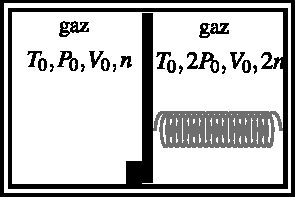
\includegraphics[width=\linewidth]{etat_fin-plain}
		\end{center}
	\end{minipage}
}%
\QR{%
	Décrire qualitativement l'évolution du système.
}{%
	solu
}%
\QR{%
	Écrire cinq relations faisant intervenir certaines des six variables d'état~:
	$V_1$ et $V_2$ les volumes finaux de chaque compartiment, $P_1$ et $P_2$ leurs
	pressions, et $T_1$ et $T_2$ leurs températures.
}{%
	solu
}%

\end{document}
